\begin{filecontents*}{because_sources.bib}
@book{weinberg1992,
  author    = {Steven Weinberg},
  title     = {Dreams of a Final Theory: The Scientist's Search for the Ultimate Laws of Nature},
  year      = {1992},
  publisher = {Pantheon Books},
  address   = {New York},
  isbn      = {9780679419235}
}

@book{huxley1868,
  author    = {Thomas Henry Huxley},
  title     = {On a Piece of Chalk: A Lecture to Working Men},
  year      = {1868},
  publisher = {Macmillan},
  address   = {London},
  url       = {https://www.gutenberg.org/ebooks/1315}
}

@book{bohren1983,
  author    = {Craig F. Bohren and Donald R. Huffman},
  title     = {Absorption and Scattering of Light by Small Particles},
  year      = {1983},
  publisher = {John Wiley \& Sons},
  address   = {New York},
  doi       = {10.1002/9783527618156}
}

@article{smith2005,
  author  = {Glenn S. Smith},
  title   = {Human Color Vision and the Unsaturated Blue Color of the Daytime Sky},
  journal = {American Journal of Physics},
  year    = {2005},
  volume  = {73},
  number  = {7},
  pages   = {590--597},
  doi     = {10.1119/1.1858479}
}

@article{popefry1997,
  author  = {Robin M. Pope and Edward S. Fry},
  title   = {Absorption Spectrum (380--700 nm) of Pure Water. {II}. Integrating Cavity Measurements},
  journal = {Applied Optics},
  year    = {1997},
  volume  = {36},
  number  = {33},
  pages   = {8710--8723},
  doi     = {10.1364/AO.36.008710}
}

@article{morel1977,
  author  = {Andr\'e Morel and Louis Prieur},
  title   = {Analysis of Variations in Ocean Color},
  journal = {Limnology and Oceanography},
  year    = {1977},
  volume  = {22},
  number  = {4},
  pages   = {709--722},
  doi     = {10.4319/lo.1977.22.4.0709}
}

@article{daviescolley2001,
  author  = {Robert J. Davies-Colley and David G. Smith},
  title   = {Turbidity, Suspended Sediment, and Water Clarity: A Review},
  journal = {Journal of the American Water Resources Association},
  year    = {2001},
  volume  = {37},
  number  = {5},
  pages   = {1085--1101},
  doi     = {10.1111/j.1752-1688.2001.tb03624.x}
}

@article{monteith2007,
  author  = {Donald T. Monteith and John L. Stoddard and Christopher D. Evans and Heleen A. de Wit and Martin Forsius and Tore H\aa gland and Anders Wilander and Brit Lisa Skjelkv\aa le and Dean S. Jeffries and Jussi Vuorenmaa and Bill Keller and Jiri Kop\'a\v{c}ek and Joseph Vesely},
  title   = {Dissolved Organic Carbon Trends Resulting from Changes in Atmospheric Deposition Chemistry},
  journal = {Nature},
  year    = {2007},
  volume  = {450},
  number  = {7169},
  pages   = {537--540},
  doi     = {10.1038/nature06316}
}

@article{gates1965,
  author  = {David M. Gates and Harry J. Keegan and John C. Schleter and Victor R. Weidner},
  title   = {Spectral Properties of Plants},
  journal = {Applied Optics},
  year    = {1965},
  volume  = {4},
  number  = {1},
  pages   = {11--20},
  doi     = {10.1364/AO.4.000011}
}

@article{woolley1971,
  author  = {John T. Woolley},
  title   = {Reflectance and Transmittance of Light by Leaves},
  journal = {Plant Physiology},
  year    = {1971},
  volume  = {47},
  number  = {5},
  pages   = {656--662},
  doi     = {10.1104/pp.47.5.656}
}

@article{nishio2000,
  author  = {John N. Nishio},
  title   = {Why Are Higher Plants Green? Evolution of the Higher Plant Photosynthetic Pigment Complement},
  journal = {Plant, Cell \& Environment},
  year    = {2000},
  volume  = {23},
  number  = {6},
  pages   = {539--548},
  doi     = {10.1046/j.1365-3040.2000.00563.x}
}

@article{terashima2009,
  author  = {Ichiro Terashima and Takashi Fujita and Takeshi Inoue and Wah Soon Chow and Riichi Oguchi},
  title   = {Green Light Drives Leaf Photosynthesis More Efficiently than Red Light in Strong White Light: Revisiting the Enigmatic Question of Why Leaves Are Green},
  journal = {Plant and Cell Physiology},
  year    = {2009},
  volume  = {50},
  number  = {4},
  pages   = {684--697},
  doi     = {10.1093/pcp/pcp034}
}

@article{liu2021,
  author  = {Jun Liu and Marc W. van Iersel},
  title   = {Photosynthetic Physiology of Blue, Green, and Red Light: Light Intensity Effects and Underlying Mechanisms},
  journal = {Frontiers in Plant Science},
  year    = {2021},
  volume  = {12},
  pages   = {619987},
  doi     = {10.3389/fpls.2021.619987}
}

@article{ruban2016,
  author  = {Alexander V. Ruban},
  title   = {Nonphotochemical Chlorophyll Fluorescence Quenching: Mechanism and Effectiveness in Protecting Plants from Photodamage},
  journal = {Plant Physiology},
  year    = {2016},
  volume  = {170},
  number  = {4},
  pages   = {1903--1916},
  doi     = {10.1104/pp.15.01935}
}

@article{walker2018,
  author  = {Berkley J. Walker and Darren T. Drewry and Andy Slattery and David VanLoocke and Bertrand Choquette and Christopher J. Ort and Elizabeth A. Ainsworth},
  title   = {Chlorophyll Can Be Reduced in Crop Canopies with Little Penalty to Photosynthesis},
  journal = {Plant Physiology},
  year    = {2018},
  volume  = {176},
  number  = {2},
  pages   = {1215--1232},
  doi     = {10.1104/pp.17.01401}
}

@article{arp2020,
  author  = {Trevor B. Arp and Jed Kistner-Morris and Vivek Aji and Richard J. Cogdell and Rienk van Grondelle and Nathaniel M. Gabor},
  title   = {Quieting a Noisy Antenna Reproduces Photosynthetic Light-Harvesting Spectra},
  journal = {Science},
  year    = {2020},
  volume  = {368},
  number  = {6498},
  pages   = {1490--1495},
  doi     = {10.1126/science.aba6630}
}

@article{kiang2007,
  author  = {Nancy Y. Kiang and Janet Siefert and Govindjee and Robert E. Blankenship},
  title   = {Spectral Signatures of Photosynthesis. {I}. Review of Earth Organisms},
  journal = {Astrobiology},
  year    = {2007},
  volume  = {7},
  number  = {1},
  pages   = {222--251},
  doi     = {10.1089/ast.2006.0105}
}

@article{hortensteiner2006,
  author  = {Stefan H\"ortensteiner},
  title   = {Chlorophyll Degradation during Senescence},
  journal = {Annual Review of Plant Biology},
  year    = {2006},
  volume  = {57},
  pages   = {55--77},
  doi     = {10.1146/annurev.arplant.57.032905.105212}
}

@article{hoch2001,
  author  = {William A. Hoch and Eric L. Zeldin and Brent H. McCown},
  title   = {Physiological Significance of Anthocyanins during Autumnal Leaf Senescence},
  journal = {Tree Physiology},
  year    = {2001},
  volume  = {21},
  number  = {1},
  pages   = {1--8},
  doi     = {10.1093/treephys/21.1.1}
}

@article{feild2001,
  author  = {Taylor S. Feild and David W. Lee and N. Michele Holbrook},
  title   = {Why Leaves Turn Red in Autumn: The Role of Anthocyanins in Senescing Leaves of Red-Osier Dogwood},
  journal = {Plant Physiology},
  year    = {2001},
  volume  = {127},
  number  = {2},
  pages   = {566--574},
  doi     = {10.1104/pp.010063}
}

@article{hoch2003,
  author  = {William A. Hoch and Eric L. Singsaas and Brent H. McCown},
  title   = {Resorption Protection: Anthocyanins Facilitate Nutrient Recovery in Autumn by Shielding Leaves from Potentially Damaging Light Levels},
  journal = {Plant Physiology},
  year    = {2003},
  volume  = {133},
  number  = {3},
  pages   = {1296--1305},
  doi     = {10.1104/pp.103.027631}
}

@article{archetti2000,
  author  = {Marco Archetti},
  title   = {The Origin of Autumn Colours by Coevolution},
  journal = {Journal of Theoretical Biology},
  year    = {2000},
  volume  = {205},
  number  = {4},
  pages   = {625--630},
  doi     = {10.1006/jtbi.2000.2089}
}

@article{archetti2009,
  author  = {Marco Archetti and Thomas F. D\"oring and Snorre B. Hagen and Nicole M. Hughes and Simon R. Leather and David W. Lee and Simcha Lev-Yadun and Yiannis Manetas and Helen J. Ougham and Paul G. Schaberg and Howard Thomas},
  title   = {Unravelling the Evolution of Autumn Colours: An Interdisciplinary Approach},
  journal = {Trends in Ecology \& Evolution},
  year    = {2009},
  volume  = {24},
  number  = {3},
  pages   = {166--173},
  doi     = {10.1016/j.tree.2008.10.006}
}

@article{hughes2022,
  author  = {Nicole M. Hughes and Christian O. George and Corinne B. Gumpman and Howard S. Neufeld},
  title   = {Coevolution and Photoprotection as Complementary Hypotheses for Autumn Leaf Reddening: A Nutrient-Centered Perspective},
  journal = {New Phytologist},
  year    = {2022},
  volume  = {233},
  number  = {1},
  pages   = {22--29},
  doi     = {10.1111/nph.17735}
}

@article{levyadun2022,
  author  = {Simcha Lev-Yadun},
  title   = {The Phenomenon of Red and Yellow Autumn Leaves: Hypotheses, Agreements and Disagreements},
  journal = {Journal of Evolutionary Biology},
  year    = {2022},
  volume  = {35},
  number  = {10},
  pages   = {1245--1282},
  doi     = {10.1111/jeb.14069}
}

@article{mattila2023,
  author  = {Heta Mattila and Esa Tyystj\"arvi},
  title   = {Red Pigments in Autumn Leaves of Norway Maple Do Not Offer Significant Photoprotection but Coincide with Stress Symptoms},
  journal = {Tree Physiology},
  year    = {2023},
  volume  = {43},
  number  = {5},
  pages   = {751--768},
  doi     = {10.1093/treephys/tpad010}
}

@article{mayr1961,
  author  = {Ernst Mayr},
  title   = {Cause and Effect in Biology},
  journal = {Science},
  year    = {1961},
  volume  = {134},
  number  = {3489},
  pages   = {1501--1506},
  doi     = {10.1126/science.134.3489.1501}
}

@article{tinbergen1963,
  author  = {Niko Tinbergen},
  title   = {On Aims and Methods of Ethology},
  journal = {Zeitschrift f\"ur Tierpsychologie},
  year    = {1963},
  volume  = {20},
  number  = {4},
  pages   = {410--433},
  doi     = {10.1111/j.1439-0310.1963.tb01161.x}
}

@article{haig2013,
  author  = {David Haig},
  title   = {Proximate and Ultimate Causes: How Come? and What For?},
  journal = {Biology \& Philosophy},
  year    = {2013},
  volume  = {28},
  number  = {5},
  pages   = {781--786},
  doi     = {10.1007/s10539-013-9369-z}
}

@book{dennett1995,
  author    = {Daniel C. Dennett},
  title     = {Darwin's Dangerous Idea: Evolution and the Meanings of Life},
  year      = {1995},
  publisher = {Simon \& Schuster},
  address   = {New York},
  isbn      = {9780684824710}
}

@article{kelemen1999,
  author  = {Deborah Kelemen},
  title   = {Why Are Rocks Pointy? Children's Preference for Teleological Explanations of the Natural World},
  journal = {Developmental Psychology},
  year    = {1999},
  volume  = {35},
  number  = {6},
  pages   = {1440--1452},
  doi     = {10.1037/0012-1649.35.6.1440}
}

@article{kelemen2014,
  author  = {Deborah Kelemen and Natalie A. Emmons and Rebecca Seston Schillaci and Patricia A. Ganea},
  title   = {Young Children Can Be Taught Basic Natural Selection Using a Picture-Storybook Intervention},
  journal = {Psychological Science},
  year    = {2014},
  volume  = {25},
  number  = {4},
  pages   = {893--902},
  doi     = {10.1177/0956797613516009}
}

@article{gouldlewontin1979,
  author  = {Stephen Jay Gould and Richard C. Lewontin},
  title   = {The Spandrels of San Marco and the Panglossian Paradigm: A Critique of the Adaptationist Programme},
  journal = {Proceedings of the Royal Society of London. Series B, Biological Sciences},
  year    = {1979},
  volume  = {205},
  number  = {1161},
  pages   = {581--598},
  doi     = {10.1098/rspb.1979.0086}
}

@article{hubalek2020,
  author  = {Michal Hub\'alek},
  title   = {A Brief (Hi)story of Just-So Stories in Evolutionary Science},
  journal = {Philosophy of the Social Sciences},
  year    = {2020},
  volume  = {50},
  number  = {6},
  pages   = {569--596},
  doi     = {10.1177/0048393120944223}
}

@book{kipling1902,
  author    = {Rudyard Kipling},
  title     = {Just So Stories for Little Children},
  year      = {1902},
  publisher = {Macmillan},
  address   = {London},
  url       = {https://www.gutenberg.org/ebooks/2781}
}

@book{deutsch2011,
  author    = {David Deutsch},
  title     = {The Beginning of Infinity: Explanations That Transform the World},
  year      = {2011},
  publisher = {Viking},
  address   = {New York},
  isbn      = {9780670022755}
}

@book{feynman1963,
  author    = {Richard P. Feynman and Robert B. Leighton and Matthew Sands},
  title     = {The Feynman Lectures on Physics, Volume I},
  year      = {1963},
  publisher = {Addison-Wesley},
  address   = {Reading, Massachusetts},
  note      = {Chapter 3, ``The Relation of Physics to Other Sciences''},
  url       = {https://www.feynmanlectures.caltech.edu/I_03.html}
}

@book{gould1989,
  author    = {Stephen Jay Gould},
  title     = {Wonderful Life: The Burgess Shale and the Nature of History},
  year      = {1989},
  publisher = {W. W. Norton},
  address   = {New York},
  isbn      = {9780393027051}
}

@article{blount2008,
  author  = {Zachary D. Blount and Christina Z. Borland and Richard E. Lenski},
  title   = {Historical Contingency and the Evolution of a Key Innovation in an Experimental Population of {Escherichia coli}},
  journal = {Proceedings of the National Academy of Sciences of the United States of America},
  year    = {2008},
  volume  = {105},
  number  = {23},
  pages   = {7899--7906},
  doi     = {10.1073/pnas.0803151105}
}

@article{ford2008,
  author  = {Michael J. Ford},
  title   = {Disciplinary Authority and Accountability in Scientific Practice and Learning},
  journal = {Science Education},
  year    = {2008},
  volume  = {92},
  number  = {3},
  pages   = {404--423},
  doi     = {10.1002/sce.20263}
}

@article{allchin2011,
  author  = {Douglas Allchin},
  title   = {Evaluating Knowledge of the Nature of (Whole) Science},
  journal = {Science Education},
  year    = {2011},
  volume  = {95},
  number  = {3},
  pages   = {518--542},
  doi     = {10.1002/sce.20432}
}

@article{chinn2011,
  author  = {Clark A. Chinn and Luke A. Buckland and Ala Samarapungavan},
  title   = {Expanding the Dimensions of Epistemic Cognition: Arguments from Philosophy and Psychology},
  journal = {Educational Psychologist},
  year    = {2011},
  volume  = {46},
  number  = {3},
  pages   = {141--167},
  doi     = {10.1080/00461520.2011.587722}
}

@article{mcgrew2018,
  author  = {Sarah McGrew and Teresa Ortega and Joel Breakstone and Sam Wineburg},
  title   = {Can Students Evaluate Online Sources? Learning from Assessments of Civic Online Reasoning},
  journal = {Theory \& Research in Social Education},
  year    = {2018},
  volume  = {46},
  number  = {2},
  pages   = {165--193},
  doi     = {10.1080/00933104.2017.1416320}
}

@misc{feynmanbbc1983,
  author       = {Richard P. Feynman},
  title        = {Interview on Magnets and ``Why'' Questions},
  year         = {1983},
  howpublished = {BBC Horizon, \emph{Fun to Imagine}},
  note         = {Magnets segment; the Aunt Minnie and ice passage}
}

@article{rosenberg2005,
  author  = {Robert Rosenberg},
  title   = {Why Is Ice Slippery?},
  journal = {Physics Today},
  year    = {2005},
  volume  = {58},
  number  = {12},
  pages   = {50--55},
  doi     = {10.1063/1.2169444}
}

@article{dash2006,
  author  = {J. G. Dash and A. W. Rempel and J. S. Wettlaufer},
  title   = {The Physics of Premelted Ice and Its Geophysical Consequences},
  journal = {Reviews of Modern Physics},
  year    = {2006},
  volume  = {78},
  number  = {3},
  pages   = {695--741},
  doi     = {10.1103/RevModPhys.78.695}
}

@article{weber2018,
  author  = {Bart Weber and Yuki Nagata and Stefania Ketzetzi and Fujie Tang and Wilbert J. Smit and Huib J. Bakker and Ellen H. G. Backus and Mischa Bonn and Daniel Bonn},
  title   = {Molecular Insight into the Slipperiness of Ice},
  journal = {The Journal of Physical Chemistry Letters},
  year    = {2018},
  volume  = {9},
  number  = {11},
  pages   = {2838--2842},
  doi     = {10.1021/acs.jpclett.8b01188}
}

@article{canale2019,
  author  = {L. Canale and J. Comtet and A. Nigu\`es and C. Cohen and C. Clanet and A. Siria and L. Bocquet},
  title   = {Nanorheology of Interfacial Water during Ice Gliding},
  journal = {Physical Review X},
  year    = {2019},
  volume  = {9},
  number  = {4},
  pages   = {041025},
  doi     = {10.1103/PhysRevX.9.041025}
}

@article{bowden1939,
  author  = {F. P. Bowden and T. P. Hughes},
  title   = {The Mechanism of Sliding on Ice and Snow},
  journal = {Proceedings of the Royal Society of London. Series A},
  year    = {1939},
  volume  = {172},
  number  = {949},
  pages   = {280--298}
}

@article{kirschner2006,
  author  = {Paul A. Kirschner and John Sweller and Richard E. Clark},
  title   = {Why Minimal Guidance during Instruction Does Not Work: An Analysis of the Failure of Constructivist, Discovery, Problem-Based, Experiential, and Inquiry-Based Teaching},
  journal = {Educational Psychologist},
  year    = {2006},
  volume  = {41},
  number  = {2},
  pages   = {75--86},
  doi     = {10.1207/s15326985ep4102_1}
}

@article{hmelosilver2007,
  author  = {Cindy E. Hmelo-Silver and Ravit Golan Duncan and Clark A. Chinn},
  title   = {Scaffolding and Achievement in Problem-Based and Inquiry Learning: A Response to Kirschner, Sweller, and Clark (2006)},
  journal = {Educational Psychologist},
  year    = {2007},
  volume  = {42},
  number  = {2},
  pages   = {99--107},
  doi     = {10.1080/00461520701263368}
}

@misc{bsb2026,
  author       = {{Bar Standards Board}},
  title        = {The {BSB} Handbook},
  year         = {2026},
  howpublished = {Version 4.9, Part 2: Code of Conduct},
  note         = {Core Duty 1; rule rC3.4 and guidance gC5 on adverse authority},
  url          = {https://www.barstandardsboard.org.uk/the-bsb-handbook.html}
}

@article{strutt1871,
  author  = {John William Strutt},
  title   = {On the Light from the Sky, Its Polarization and Colour},
  journal = {The London, Edinburgh, and Dublin Philosophical Magazine and Journal of Science},
  year    = {1871},
  volume  = {41},
  number  = {271},
  pages   = {107--120}
}

@article{hulburt1953,
  author  = {E. O. Hulburt},
  title   = {Explanation of the Brightness and Color of the Sky, Particularly the Twilight Sky},
  journal = {Journal of the Optical Society of America},
  year    = {1953},
  volume  = {43},
  number  = {2},
  pages   = {113--118},
  doi     = {10.1364/JOSA.43.000113}
}

@article{lange2023,
  author  = {Anna Lange and Alexei Rozanov and Christian von Savigny},
  title   = {Revisiting the Question ``Why Is the Sky Blue?''},
  journal = {Atmospheric Chemistry and Physics},
  year    = {2023},
  volume  = {23},
  number  = {23},
  pages   = {14829--14839},
  doi     = {10.5194/acp-23-14829-2023}
}

@article{wehner2006,
  author  = {R\"udiger Wehner and Martin M\"uller},
  title   = {The Significance of Direct Sunlight and Polarized Skylight in the Ant's Celestial System of Navigation},
  journal = {Proceedings of the National Academy of Sciences of the United States of America},
  year    = {2006},
  volume  = {103},
  number  = {33},
  pages   = {12575--12579},
  doi     = {10.1073/pnas.0604430103}
}

@book{lythgoe1979,
  author    = {John N. Lythgoe},
  title     = {The Ecology of Vision},
  year      = {1979},
  publisher = {Clarendon Press},
  address   = {Oxford}
}

@article{mollon1989,
  author  = {J. D. Mollon},
  title   = {``Tho' She Kneel'd in That Place Where They Grew'': The Uses and Origins of Primate Colour Vision},
  journal = {Journal of Experimental Biology},
  year    = {1989},
  volume  = {146},
  pages   = {21--38}
}

@article{lovelock1974,
  author  = {James E. Lovelock and Lynn Margulis},
  title   = {Atmospheric Homeostasis by and for the Biosphere: The Gaia Hypothesis},
  journal = {Tellus},
  year    = {1974},
  volume  = {26},
  number  = {1--2},
  pages   = {2--10},
  doi     = {10.3402/tellusa.v26i1-2.9731}
}

@article{watson1983,
  author  = {Andrew J. Watson and James E. Lovelock},
  title   = {Biological Homeostasis of the Global Environment: The Parable of Daisyworld},
  journal = {Tellus B},
  year    = {1983},
  volume  = {35},
  number  = {4},
  pages   = {284--289},
  doi     = {10.3402/tellusb.v35i4.14616}
}

@article{lenton2018,
  author  = {Timothy M. Lenton and Stuart J. Daines and James G. Dyke and Arwen E. Nicholson and David M. Wilkinson and Hywel T. P. Williams},
  title   = {Selection for Gaia across Multiple Scales},
  journal = {Trends in Ecology \& Evolution},
  year    = {2018},
  volume  = {33},
  number  = {8},
  pages   = {633--645},
  doi     = {10.1016/j.tree.2018.05.006}
}

@article{doolittle2017,
  author  = {W. Ford Doolittle and Austin Booth},
  title   = {It's the Song, Not the Singer: An Exploration of Holobiosis and Evolutionary Theory},
  journal = {Biology \& Philosophy},
  year    = {2017},
  volume  = {32},
  number  = {1},
  pages   = {5--24},
  doi     = {10.1007/s10539-016-9542-2}
}

@article{doolittle2018,
  author  = {W. Ford Doolittle and S. Andrew Inkpen},
  title   = {Processes and Patterns of Interaction as Units of Selection: An Introduction to {ITSNTS} Thinking},
  journal = {Proceedings of the National Academy of Sciences of the United States of America},
  year    = {2018},
  volume  = {115},
  number  = {16},
  pages   = {4006--4014},
  doi     = {10.1073/pnas.1722232115}
}

@book{godfreysmith2009,
  author    = {Peter Godfrey-Smith},
  title     = {Darwinian Populations and Natural Selection},
  year      = {2009},
  publisher = {Oxford University Press},
  address   = {Oxford}
}

@book{okasha2006,
  author    = {Samir Okasha},
  title     = {Evolution and the Levels of Selection},
  year      = {2006},
  publisher = {Oxford University Press},
  address   = {Oxford}
}

@book{odlingsmee2003,
  author    = {F. John Odling-Smee and Kevin N. Laland and Marcus W. Feldman},
  title     = {Niche Construction: The Neglected Process in Evolution},
  year      = {2003},
  publisher = {Princeton University Press},
  address   = {Princeton}
}

@book{einstein1950,
  author    = {Albert Einstein},
  title     = {Out of My Later Years},
  year      = {1950},
  publisher = {Philosophical Library},
  address   = {New York},
  note      = {Chapter 9, ``On Education'', from the address to the Convocation of the State University of New York at Albany, 15 October 1936}
}

@misc{qi2014,
  author       = {{Quote Investigator}},
  title        = {Education Is What Remains After You Have Forgotten Everything You Learned in School},
  year         = {2014},
  howpublished = {Quote Investigator},
  note         = {Accessed 18 September 2026},
  url          = {https://quoteinvestigator.com/2014/09/07/forgotten/}
}

@book{baum1900,
  author    = {L. Frank Baum},
  title     = {The Wonderful Wizard of Oz},
  year      = {1900},
  publisher = {George M. Hill Company},
  address   = {Chicago}
}
\end{filecontents*}

\documentclass[11pt,a4paper]{article}
\usepackage[margin=23mm,headheight=22pt]{geometry}
\usepackage[T1]{fontenc}
\usepackage{lmodern}
\usepackage{microtype}
\usepackage{xcolor}
\usepackage{graphicx}
\usepackage{booktabs}
\usepackage{tabularx}
\usepackage{array}
\usepackage{enumitem}
\usepackage{tikz}
\usetikzlibrary{arrows.meta,positioning,calc,decorations.pathmorphing}
\usepackage[most]{tcolorbox}
\usepackage{amsmath}
\usepackage{natbib}
\usepackage{xurl}
\usepackage{hyperref}
\usepackage{fancyhdr}
\usepackage{titlesec}
\usepackage{multicol}
\usepackage{needspace}
\usepackage{doi}

\definecolor{night}{HTML}{183044}
\definecolor{sky}{HTML}{4D8FB5}
\definecolor{water}{HTML}{287F86}
\definecolor{leaf}{HTML}{3D7556}
\definecolor{autumn}{HTML}{9B453C}
\definecolor{ochre}{HTML}{B4782D}
\definecolor{chalk}{HTML}{F7F3E8}
\definecolor{mist}{HTML}{EEF4F3}
\definecolor{ink}{HTML}{1D292D}
\definecolor{slate}{HTML}{58666B}
\definecolor{linegrey}{HTML}{CCD6D4}
\definecolor{palegreen}{HTML}{EDF4EE}
\definecolor{paleblue}{HTML}{EDF4F8}
\definecolor{palered}{HTML}{F8EFEC}

\hypersetup{
  colorlinks=true,
  linkcolor=night,
  citecolor=autumn,
  urlcolor=water,
  pdftitle={The Cheapness of Because},
  pdfauthor={Lee McCulloch-James (McMurmerings)},
  pdfsubject={Accountable authority, scientific explanation, and classroom provenance},
  pdfkeywords={science education, explanation, provenance, teleology, contingency, leaves, water, sky, chalk}
}

\pagestyle{fancy}
\fancyhf{}
\fancyhead[L]{\small\color{slate}\MakeUppercase{The cheapness of because}}
\fancyhead[R]{\small\color{slate}ACCOUNTABLE AUTHORITY IN SCIENCE TEACHING}
\fancyfoot[L]{\scriptsize\color{slate}\housestamp}
\fancyfoot[R]{\small\color{slate}\thepage}
\renewcommand{\headrulewidth}{0.45pt}
\renewcommand{\headrule}{\hbox to\headwidth{\color{linegrey}\leaders\hrule height \headrulewidth\hfill}}
\renewcommand{\footrulewidth}{0pt}

\titleformat{\section}{\Large\bfseries\color{night}}{\thesection}{0.7em}{}
\titleformat{\subsection}{\large\bfseries\color{water}}{\thesubsection}{0.6em}{}
\titleformat{\subsubsection}{\normalsize\bfseries\color{leaf}}{\thesubsubsection}{0.55em}{}
\titlespacing*{\section}{0pt}{2.5ex plus .8ex minus .3ex}{1.05ex}
\titlespacing*{\subsection}{0pt}{1.9ex plus .5ex minus .2ex}{.65ex}
\titlespacing*{\subsubsection}{0pt}{1.4ex plus .4ex minus .2ex}{.4ex}

\setlength{\parindent}{0pt}
\setlength{\parskip}{0.62em}
\setlist{nosep,leftmargin=1.45em,topsep=.35em}
\raggedbottom
\clubpenalty=10000
\widowpenalty=10000
\displaywidowpenalty=10000

\newcommand{\grade}[2]{\textbf{\textcolor{#1}{#2}}}
\newcommand{\casehead}[2]{\textcolor{#1}{\textbf{#2}}}
\newcommand{\term}[1]{\textbf{\textcolor{night}{#1}}}
\newcommand{\housestamp}{Constructed by Silicon \textperiodcentered\ Anthropic Claude \textemdash\ Architect Carbon \textperiodcentered\ LeeMcCullochJames}

\newtcolorbox{thesisbox}[1][]{
  enhanced,breakable,colback=mist,colframe=water,boxrule=.85pt,arc=2mm,
  left=3.5mm,right=3.5mm,top=2.6mm,bottom=2.6mm,
  fonttitle=\bfseries,title={The argument in one paragraph},#1}

\newtcolorbox{compressed}[1][]{
  enhanced,breakable,colback=chalk,colframe=ochre,boxrule=.75pt,arc=2mm,
  left=3mm,right=3mm,top=2.2mm,bottom=2.2mm,
  fonttitle=\bfseries,title={A useful compression},#1}

\newtcolorbox{decompress}[1][]{
  enhanced,breakable,colback=paleblue,colframe=sky,boxrule=.75pt,arc=2mm,
  left=3mm,right=3mm,top=2.2mm,bottom=2.2mm,
  fonttitle=\bfseries,title={Decompression handle},#1}

\newtcolorbox{provenance}[1][]{
  enhanced,breakable,colback=palered,colframe=autumn,boxrule=.75pt,arc=2mm,
  left=3mm,right=3mm,top=2.2mm,bottom=2.2mm,
  fonttitle=\bfseries,title={Provenance check},#1}

\newtcolorbox{openquestion}[1][]{
  enhanced,breakable,colback=white,colframe=leaf,boxrule=.75pt,arc=2mm,
  left=3mm,right=3mm,top=2.2mm,bottom=2.2mm,
  fonttitle=\bfseries,title={Question left open},#1}

\begin{document}
\pagenumbering{roman}

\begin{titlepage}
\thispagestyle{empty}

\begin{tikzpicture}[remember picture,overlay]
  \fill[chalk] (current page.south west) rectangle (current page.north east);
  \fill[night] (current page.north west) rectangle ([yshift=-25mm]current page.north east);
  \fill[sky] ([yshift=-25mm]current page.north west) rectangle ([yshift=-32mm]current page.north east);
  \fill[water] ([yshift=-32mm]current page.north west) rectangle ([yshift=-39mm]current page.north east);
  \fill[leaf] ([yshift=-39mm]current page.north west) rectangle ([yshift=-46mm]current page.north east);
  \fill[autumn] ([yshift=-46mm]current page.north west) rectangle ([yshift=-53mm]current page.north east);
  \draw[ochre,line width=1pt] ([xshift=24mm,yshift=28mm]current page.south west) -- ([xshift=-24mm,yshift=28mm]current page.south east);
\end{tikzpicture}

\vspace*{41mm}
\begin{minipage}{.9\textwidth}
{\small\bfseries\color{water}\MakeUppercase{Chalk, sky, water, leaves, and the provenance of explanation}}\\[7mm]
{\fontsize{32}{37}\selectfont\bfseries\color{night}The Cheapness of Because}\\[4mm]
{\Large\color{ink}How teachers can compress science without closing inquiry}\\[12mm]

\begin{tcolorbox}[colback=white,colframe=linegrey,boxrule=.8pt,arc=2mm,left=4mm,right=4mm,top=3.5mm,bottom=3.5mm]
\large
A school explanation is necessarily smaller than the science behind it, so the ethical and intellectual question concerns whether the compression carries its provenance, its boundary, and a route back into inquiry. Once explanations cost nothing to obtain, the teacher's work shifts from conveying them towards arguing for what deserves weight, and that shift brings duties with it.
\end{tcolorbox}

\vfill
{\normalsize\color{slate}
Lee McCulloch-James \textperiodcentered\ McMurmerings\\
An essay for science teachers and upper-secondary students\\
Research audit: 18 September 2026\\[2mm]
Full journal references, evidence grades, and classroom protocols included\\[4mm]
\scriptsize\housestamp
}
\end{minipage}
\end{titlepage}

\pagenumbering{arabic}

\begin{thesisbox}
Teachers exercise authority whether or not they claim it, since they choose what enters the lesson, in what order, at what resolution, and under which verb, whether \emph{is}, \emph{causes}, \emph{suggests}, or \emph{evolved for}. When descriptions were scarce that work resembled conveyancing, the careful transfer of a title somebody else had established; now that fluent explanation is free, the scarce goods are discernment and research acumen, and the labour drifts towards advocacy, which is the barrister's craft and carries the barrister's duties. Authority becomes accountable when a compact explanation reveals what kind of answer it is, what evidence warrants it, where it ceases to work, what remains disputed, and which evidence runs against the case being made. The cases in this essay move from chalk to sky, water, green leaves, autumn-red leaves, and the ice on which Feynman's Aunt Minnie slipped. Together they show that physics and chemistry constrain; geology supplies paths, materials, and accidents; biology inherits and modifies; observers classify; and no single ``because'' is entitled to perform all of those explanatory jobs at once.
\end{thesisbox}

\begingroup
\small
\setlength{\parskip}{0pt}
\tableofcontents
\endgroup
\clearpage

\section{The cheapness of \emph{because}}

Explanations have become easy to obtain. A search box, textbook margin, video, or generative system can produce a polished paragraph before a learner has decided what was being asked. Fluency has become cheap; warrants have not. Misinformation is the obvious hazard and the smaller one, since the subtler danger is a true sentence arriving with the shape and confidence of a complete idea.

``The sky is blue because blue light is scattered more.'' ``Water is transparent.'' ``Leaves are green because chlorophyll reflects green.'' Each can be useful at the right moment. Each can also create what might be called \term{epistemic compression with concealed seams}: a small description that suppresses its scale, assumptions, observer, history, and evidential status, then passes as the finished account.

Compression is unavoidable, since a map omitting nothing would be useless and a lesson containing every qualification would never begin. The useful contrast therefore runs between a \emph{sealed} compression and a \emph{provenance-bearing} one, with simplification common to both.

\begin{center}
\small
\renewcommand{\arraystretch}{1.25}
\begin{tabularx}{.96\linewidth}{>{\bfseries\color{autumn}}p{.20\linewidth}X X}
\toprule
& \textbf{Sealed compression} & \textbf{Provenance-bearing compression} \\
\midrule
Claim & Sounds complete; often contains an unmarked ``always'', ``only'', or ``for''. & States the smallest defensible proposition. \\
Evidence & Hides behind the teacher, textbook, or confident tone. & Names the kind of evidence and, where useful, the source chain. \\
Boundary & Treats exceptions as nuisances. & Says which scale, system, and conditions the claim covers. \\
Uncertainty & Either erases it or makes all knowledge sound doubtful. & Separates secure mechanism, bounded generalisation, and open history. \\
Invitation & Rewards reproduction of the vignette. & Supplies a handle by which the learner can reopen it. \\
\bottomrule
\end{tabularx}
\end{center}

A good short explanation closes one question securely enough to expose the next, giving curiosity traction instead of feeding it until it falls quiet.

\section{The teacher as an accountable authority}

The legal word \emph{conveyancer} is suggestive. A conveyancer does not create the land being transferred; the work is to establish what is being conveyed, under what title, with which boundaries and encumbrances. Teachers likewise do not manufacture the authority of a spectrometer, field comparison, experiment, or scholarly community. They select and convey claims. The classroom version of a clean chain of title is \term{provenance}: who claims this, on what evidence, through which transformations, with what reach?

The analogy has limits, but it rescues two truths often pulled apart. First, teachers genuinely exercise authority. They choose examples, omit detail, sequence concepts, translate vocabulary, and decide what counts as an adequate answer. Second, scientific authority is never a personal possession, remaining answerable throughout to methods, evidence, criticism, and the possibility of revision. Ford calls attention to this relation between disciplinary authority and accountability; Allchin similarly argues for teaching the practices and social architecture of ``whole science'', not only finished products \citep{ford2008,allchin2011}.

Accountability has little to do with a performance of hesitation, since ``scientists are not sure'' is a poor refrain when the relevant mechanism is secure, and staging every established result as a live debate misleads in the opposite direction. The teacher's task is more exacting, in that confidence should change when the proposition changes.

\begin{center}
\small
\renewcommand{\arraystretch}{1.25}
\begin{tabularx}{.94\linewidth}{>{\bfseries\color{night}}p{.22\linewidth}>{\raggedright\arraybackslash}p{.27\linewidth}X}
\toprule
\textbf{Claim type} & \textbf{Typical evidence} & \textbf{Responsible classroom voice} \\
\midrule
Observation & Calibrated measurement; repeated description & ``Under these conditions, we observe\ldots'' \\
Mechanism & Intervention, model, physical or chemical constraint & ``This occurs through\ldots'' \\
Historical route & Geological trace, phylogeny, archival record, converging reconstruction & ``The best-supported sequence is\ldots'' \\
Current role & Manipulation and measured consequence in a living system & ``In this system, the feature can\ldots'' \\
Selected function & Comparative and fitness evidence tied to ancestral alternatives & ``Evidence suggests selection favoured\ldots'' \\
Intended purpose & Evidence of an agent, plan, or interpretation & ``This was designed or used in order to\ldots'' \\
\bottomrule
\end{tabularx}
\end{center}

The distinctions matter because the word \emph{because} can quietly move a class from one row to another. A mechanism becomes a history; a beneficial effect becomes the reason a trait originated; regularity becomes intention.

\section{The conveyancer and the advocate}

The conveyancing analogy carries a hidden assumption about scarcity, since conveyancing matters in a world where establishing and transferring a title is the difficult part of the transaction. A classroom once sat in that world: the textbook was the deed, the teacher established what it said and passed it on intact, and a pupil who received the description accurately had received something not easily obtained elsewhere. Description now costs nothing. A phone produces a fluent paragraph on chlorophyll, regelation, or ocean colour in the time it takes to ask, and the paragraph is frequently correct.

What remains scarce is discernment, meaning the capacity to tell which of four plausible paragraphs deserves weight, which question each of them is answering, and what would have to be true for one of them to fail. Conveying no longer exhausts the work, and the part that has grown is persuasion, since a learner who cannot yet evaluate a claim must nonetheless be brought to treat some claims as more trustworthy than others. That is the barrister's function, and the drift towards it is worth naming plainly, given that the profession's preferred self-image is the honest broker who merely transmits.

The self-image was always partly a fiction. A teacher who selects the example, fixes the sequence, chooses which caveat to omit, decides what counts as a sufficient answer, and delivers a contested claim in a settled tone has been making a case all along, with the label withheld. The honest response is to accept the advocacy and import the constraints that make advocacy respectable, since denying it loses the constraints along with the label.

Those constraints are unusually well codified. A barrister in England and Wales owes an overriding duty to the court to act with independence in the interests of justice, a duty that displaces inconsistent obligations to the client; the advocate must not knowingly or recklessly mislead, and must take reasonable steps to ensure that the court has before it all relevant decisions and provisions, which the accompanying guidance makes explicit includes authority adverse to the client's own case \citep{bsb2026}. Translated into a classroom, the second obligation is the demanding one. A teacher may argue for a conclusion, and having argued for it owes the class the strongest evidence running the other way, supplied unprompted rather than extracted under questioning. That single duty separates a case from a sales pitch.

The other half of advocacy is examination, which is the half a classroom most needs now. A generated paragraph arrives with the fluency of testimony and none of the exposure, since nobody has asked it what it is in a position to know, how it came to know it, what it would have said had the evidence pointed elsewhere, or whose account it is reproducing. Students can learn to put those questions to a source in the way counsel puts them to a witness, and the questions transfer intact to textbooks, to teachers, and to the students' own paragraphs.

\begin{center}
\small
\renewcommand{\arraystretch}{1.24}
\begin{tabularx}{\linewidth}{>{\bfseries\color{night}}p{.19\linewidth}>{\raggedright\arraybackslash}p{.33\linewidth}X}
\toprule
\textbf{Role} & \textbf{What it supplies} & \textbf{Characteristic failure} \\
\midrule
Conveyancer & An accurate title: what the claim says, with its boundaries and encumbrances & Treating transfer as the whole task once transfer has become free \\
\addlinespace
Advocate & A case for what deserves weight, with the adverse authority disclosed & Persuasion that withholds the contrary evidence and calls the omission simplification \\
\addlinespace
Examiner & Pressure applied to a source: what it knows, how it knows, and what would change it & Scepticism practised as a mannerism, applied evenly to strong and weak claims alike \\
\bottomrule
\end{tabularx}
\end{center}

The analogy has limits that deserve stating, since a courtroom supplies an opposing counsel, a tribunal, rules of evidence, and a verdict, while a classroom supplies one voice, a timetable, and an examination board whose mark scheme frequently rewards the sealed vignette. A teacher who ignores the mark scheme damages students in a way that no epistemic virtue repays, and a teacher who obeys it completely reproduces the very thing this essay complains about. The workable compromise is to teach the mark-scheme sentence as what it is, an instrument calibrated for a marker, and then to spend a small protected fraction of the lesson reopening it, which costs minutes rather than schemes of work.

The following objects make those migrations visible.

\section{Chalk: Weinberg's descent and Huxley's return}

Steven Weinberg begins Chapter 2 of \emph{Dreams of a Final Theory} with an ordinary piece of chalk. The chapter is ``On a Piece of Chalk'', not a passage from \emph{The First Three Minutes}; the bibliographic correction is apt in an essay about provenance \citep{weinberg1992}. His title in turn recalls T.~H. Huxley's nineteenth-century lecture, which read geological and biological history from chalk \citep{huxley1868}.

Why is chalk white? A compact causal descent might run as follows.

\begin{center}
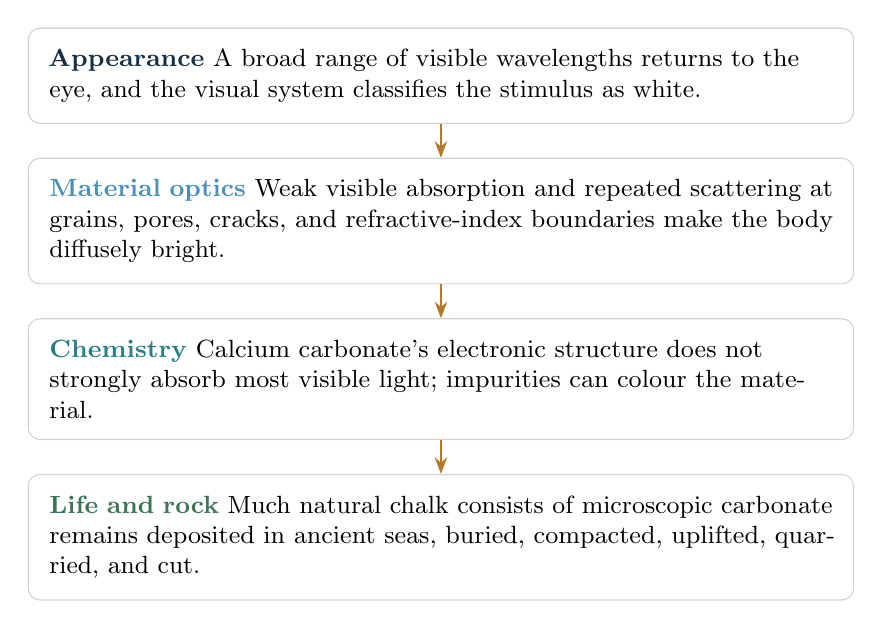
\begin{tikzpicture}[
  node distance=4.3mm,
  every node/.style={font=\small,align=left},
  box/.style={draw=linegrey,fill=white,rounded corners=1.5mm,text width=.82\linewidth,inner sep=2.7mm},
  arr/.style={-{Stealth[length=2.1mm]},draw=ochre,line width=.85pt}
]
\node[box] (a) {\casehead{night}{Appearance} A broad range of visible wavelengths returns to the eye, and the visual system classifies the stimulus as white.};
\node[box,below=of a] (b) {\casehead{sky}{Material optics} Weak visible absorption and repeated scattering at grains, pores, cracks, and refractive-index boundaries make the body diffusely bright.};
\node[box,below=of b] (c) {\casehead{water}{Chemistry} Calcium carbonate's electronic structure does not strongly absorb most visible light; impurities can colour the material.};
\node[box,below=of c] (d) {\casehead{leaf}{Life and rock} Much natural chalk consists of microscopic carbonate remains deposited in ancient seas, buried, compacted, uplifted, quarried, and cut.};
\draw[arr] (a)--(b); \draw[arr] (b)--(c); \draw[arr] (c)--(d);
\end{tikzpicture}
\end{center}

Scattering and absorption can be connected to electromagnetism, quantum transitions, particle size, and refractive index \citep{bohren1983}. But those laws do not state that this hand specimen had to exist. For that, the explanation turns outward: organisms precipitated carbonate; ecological conditions allowed deposits to accumulate; tectonics and erosion exposed them; human practices placed a fragment in a classroom.

This is reduction without erasure. The deeper physics constrains every link, yet a quantum account does not replace sedimentology, evolutionary history, or quarrying. Huxley reads upward from the object into history; Weinberg reads downward towards more general law. A complete explanation needs both movements.

\begin{compressed}
Chalk looks white because it absorbs little visible light and multiply scatters many visible wavelengths back towards the observer.
\end{compressed}

\begin{decompress}
Why does the microstructure scatter so effectively? Why is the mineral there? Which living processes supplied it? Which geological events made this sample available? The first answer remains true when these questions are opened; it simply stops pretending to be the whole biography.
\end{decompress}

\section{Blue sky: a mechanism that still needs an observer}

The canonical school answer is Rayleigh scattering. When particles are much smaller than visible wavelengths, shorter wavelengths are scattered much more strongly; in the idealised regime the dependence is approximately

\begin{equation*}
I_{\mathrm{scattered}} \propto \lambda^{-4}.
\end{equation*}

That relation, which Rayleigh derived and then used to account for both the colour and the polarisation of skylight \citep{strutt1871}, is indispensable, and it is not yet a colour. Daylight has a spectrum; the atmosphere has gases, aerosols, clouds, density gradients, and paths of different length; the observer looks in a particular direction; and a visual system maps the arriving spectrum onto perceptual categories.

\subsection{Why not violet? Three repairs in three different places}

The obvious follow-up is the most useful question a class can put to the standard answer. If scattering rises as $\lambda^{-4}$, then violet light near $400\ \mathrm{nm}$ is scattered about $1.7$ times as strongly as blue light near $460\ \mathrm{nm}$, and roughly nine times as strongly as red light near $700\ \mathrm{nm}$, so the sky ought on that reasoning to appear violet. It does not, and the repairs required sit at three different points in the chain, which is the reason no single replacement sentence does the job.

\begin{enumerate}[label=\textbf{\arabic*.}]
  \item \term{The illuminant is not flat.} The $\lambda^{-4}$ factor multiplies the solar spectrum reaching the atmosphere, and that spectrum is already falling away at the short-wave end, with ozone and other absorbers removing more of it before scattering occurs. The scattered radiance therefore still climbs towards the violet, and it climbs a good deal less steeply than the scattering law alone suggests.

  \item \term{The medium subtracts as well as scatters.} Ozone absorbs weakly across the orange and red through its Chappuis band, which removes long-wave light from the transmitted beam and deepens the blue that remains. Hulburt calculated in 1953 that the blue of the zenith sky with the Sun at the horizon owes about one third to Rayleigh scattering and two thirds to ozone absorption \citep{hulburt1953}, and a recent radiative-transfer study using the CIE colour system reproduces his estimate at the horizon while showing that the ozone contribution is minor for a high Sun and grows with solar zenith angle, viewing zenith angle, and total ozone column \citep{lange2023}. The blue of a summer midday and the blue of the blue hour are therefore not the same phenomenon, and the textbook sentence quietly runs them together.

  \item \term{A spectrum has a peak; a colour has coordinates.} This is the load-bearing error in the puzzle. The sky delivers a broad stimulus rather than a spectral line, and the visual system reduces that stimulus to three cone responses before any question of hue arises. Violet light excites the short-wave cones and, through the secondary rise in its sensitivity at short wavelengths, the long-wave cones as well, so a violet-weighted broadband stimulus maps to a desaturated blue; luminous efficiency also falls steeply below $450\ \mathrm{nm}$, and multiple scattering, haze, and ground reflection add broadband light that carries the stimulus further towards white. Smith's colorimetric treatment carries this through to the chromaticity of the daylight sky, which lands well inside the blue region and well short of the spectrum locus \citep{smith2005}.
\end{enumerate}

The third repair is worth dwelling on, since the same confusion returns later in this essay when a solar spectrum is laid beside a chlorophyll absorption curve. Asking which wavelength is most abundant, and asking what colour a mixture appears, are questions about different objects, and a graph answers only the first.

\begin{center}
\small
\renewcommand{\arraystretch}{1.24}
\begin{tabularx}{\linewidth}{>{\bfseries\color{sky}}p{.20\linewidth}>{\raggedright\arraybackslash}p{.26\linewidth}X}
\toprule
\textbf{Repair} & \textbf{Where it acts} & \textbf{What it changes about the answer} \\
\midrule
Source spectrum & Before scattering & The quantity being multiplied by $\lambda^{-4}$ is already declining in the violet \\
\addlinespace
Ozone absorption & Along the path & Long-wave light is removed; the effect is small overhead and dominant at twilight \citep{hulburt1953,lange2023} \\
\addlinespace
Trichromatic encoding & At the observer & A broadband stimulus becomes three numbers, and violet excites two channels rather than one \citep{smith2005} \\
\bottomrule
\end{tabularx}
\end{center}

\begin{equation*}
\text{sky colour} = f(\text{stellar spectrum},\ \text{atmosphere},\ \text{geometry},\ \text{observer}).
\end{equation*}

Colour is relational in consequence, which is a different matter from being merely subjective. A spectrometer can report radiance without having a colour experience; a human observer supplies a species-specific response to that radiance; and another visual system may partition the same photons differently.

\begin{provenance}
Grade the familiar sentence in parts. ``Short wavelengths are scattered more'' is established, and is the principal mechanism for a high Sun. ``Blue is scattered most'' is already careless, since violet is scattered more. ``Rayleigh scattering explains the blue of the sky'' is incomplete for the twilight zenith, where ozone absorption carries most of the effect. And no scattering law, however exact, delivers a colour without an observer to encode the spectrum.
\end{provenance}

\subsection{What a blue sky could be for}

The purpose question looks malformed, and the reason is worth stating precisely. An atmosphere has no ancestors, no heritable variation, and no differential reproduction, so there is nothing for selection to have acted upon and no selected effect to find. That verdict, however, is about the addressee of the question rather than about the question itself, because only one side of a perceptual relation has a history of selection, and it is not the sky. Eyes have ancestors.

Redirected at the receiver, the question becomes tractable and in places well evidenced. Skylight is the illuminant under which terrestrial vision evolved, and it is highly structured: a polarisation pattern fixed by scattering geometry and stable with respect to haze, a spectral difference between direct sunlight and skylight that gives shade its distinct colour, and a family of daylight spectra ordered by the Sun's elevation. Several visual systems demonstrably exploit that structure. Desert ants of the genus \emph{Cataglyphis} navigate predominantly by the skylight polarisation pattern, with the sun compass and the polarisation compass running as separate systems fed by different parts of the eye \citep{wehner2006}, and the ecological tradition in vision science treats spectral sensitivities as intelligible in relation to the light available in a habitat \citep{lythgoe1979}.

Four questions are therefore hiding inside ``what is a blue sky for'', and they have different answers:

\begin{center}
\small
\renewcommand{\arraystretch}{1.24}
\begin{tabularx}{\linewidth}{>{\bfseries\color{night}}p{.30\linewidth}>{\raggedright\arraybackslash}p{.17\linewidth}X}
\toprule
\textbf{Question} & \textbf{Answer} & \textbf{What supports it} \\
\midrule
Does the sky have a purpose or function of its own? & No & No ancestors, no heritable variation, no selection on atmospheres \\
\addlinespace
Do organisms exploit the sky's optical structure? & Yes & Behavioural and physiological evidence, as in polarisation-based navigation \citep{wehner2006} \\
\addlinespace
Was a given visual feature selected because of that structure? & Sometimes & A historical claim needing ancestral alternatives, comparative pattern, and fitness consequences \\
\addlinespace
Does a blue sky mean anything? & To interpreters & Meaning is conferred by minds and cultures, and confers nothing on the atmosphere \\
\bottomrule
\end{tabularx}
\end{center}

The third row is where the just-so risk has migrated, since a spectral sensitivity can be declared ``tuned to'' the ambient light with very little cost, and the declaration explains any tuning equally well. The history of primate trichromacy is the disciplined version of such a claim, having been argued against opsin genetics, phylogeny, and the measured spectra of the fruits and young leaves at issue, and it remains under argument \citep{mollon1989}. The requirement is the same one this essay applies to red leaves: name the ancestral alternative, and name the observation that would separate the hypotheses. Exploitation of a feature is never by itself evidence that the feature was made for the user, and the atmosphere in particular was in place long before anything looked at it.

\section{Clear water, coloured water, opaque water}

Water offers a different trap: treating transparency as a property that is either present or absent. A small clean glass can look colourless while a long path through deep water looks blue. Pure water absorbs visible light weakly and unequally across wavelengths. Careful measurements place a minimum in visible absorption in the blue region, while absorption rises towards the red; over sufficient path length, those small differences accumulate \citep{popefry1997}.

The relevant relation is attenuation:

\begin{equation*}
I(z,\lambda)=I_0(\lambda)e^{-c(\lambda)z},
\end{equation*}

where $z$ is path length and $c(\lambda)$ combines absorption and scattering out of the measured beam. Increase the distance and a weak spectral preference becomes visible. Add particles or dissolved material and the coefficients change.

Natural waters therefore carry their catchments and ecologies in their optics. Suspended mineral grains scatter; phytoplankton absorb and scatter; coloured dissolved organic matter absorbs strongly at short visible wavelengths; bubbles, bottom reflectance, surface state, and viewing angle contribute. Ocean-colour work has long separated the optical effects of water itself from those of suspended and dissolved constituents \citep{morel1977}. Reviews of turbidity likewise show why ``muddy'' cannot be reduced to one particle count or one visual impression \citep{daviescolley2001}.

\begin{center}
\small
\renewcommand{\arraystretch}{1.24}
\begin{tabularx}{\linewidth}{>{\bfseries\color{water}}p{.19\linewidth}>{\raggedright\arraybackslash}p{.28\linewidth}X}
\toprule
\textbf{Water seen} & \textbf{Important optical contributors} & \textbf{History carried into the view} \\
\midrule
Deep blue & Low particle load; preferential loss of longer visible wavelengths; molecular scattering and surface effects & Basin geometry, mixing, biological productivity, and the path through which light travels \\
Green & Phytoplankton pigments, particles, dissolved matter, and water absorption in varying proportions & Nutrient supply, seasonal growth, food webs, circulation, and catchment inputs \\
Turquoise glacial lake & Fine mineral ``flour'' strongly redistributes light & Bedrock mineralogy, glacial abrasion, meltwater routes, and particle settling \\
Tea-brown lake & Coloured dissolved organic molecules absorb blue light & Soils, vegetation, wetlands, rainfall, microbial processing, and atmospheric deposition \citep{monteith2007} \\
Opaque or turbid water & High suspended sediment, dense plankton, bubbles, or mixed loads & Erosion, floods, land use, resuspension, blooms, and basin disturbance \\
\bottomrule
\end{tabularx}
\end{center}

Is water transparent \emph{so that} life can photosynthesise? The visible transmission window is physically real and biologically consequential. Life has evolved within it and altered aquatic optics in return. But exploitation does not reverse the arrow of explanation. The molecular structure of water was not selected by aquatic organisms. A lake's present clarity can, however, be causally affected by organisms, geology, weather, and human activity. ``Physics below, biology above'' is already too static: the levels feed back.

\begin{compressed}
Pure water transmits visible light relatively well, but not equally at every wavelength; natural waters add particles and dissolved substances whose origins are geological, biological, atmospheric, and human.
\end{compressed}

\begin{decompress}
Ask for path length, wavelength, angle, constituents, and basin history, since ``transparent'' names an observation made at a particular scale, with no timeless essence behind it.
\end{decompress}

\section{Green leaves: when mechanism outruns history}

Healthy leaves commonly return a larger fraction of middle visible wavelengths to an observer than of blue and red wavelengths. Chlorophylls absorb strongly in blue and red regions; carotenoids add absorption and photoprotection; internal air--cell--water boundaries scatter light; some photons are reflected, some transmitted, and some absorbed. Classic leaf spectra make those components measurable \citep{gates1965,woolley1971}.

The familiar phrase ``chlorophyll reflects green'' is therefore a useful mnemonic with two hidden losses. A pigment primarily absorbs; a whole leaf reflects and transmits because pigments sit within structured tissue. And ``less strongly absorbed'' does not mean ``unused''. Green photons penetrate farther before absorption. Under strong white light, they can drive photosynthesis in deeper tissue more effectively at the margin than added red light, because upper chloroplasts may already be saturated \citep{terashima2009,liu2021}.

Nor is maximum capture by the first surface necessarily the biological optimum. Carbon dioxide supply, enzyme capacity, temperature, nutrient allocation, repair, and photodamage all constrain the use of excitation. In a canopy, a photon captured by a sunlit top leaf cannot reach a shaded leaf below. Models and crop measurements show conditions in which chlorophyll can be reduced with little penalty to canopy photosynthesis, although the outcome depends on architecture and environment \citep{walker2018}. Plants also regulate excess excitation through processes including nonphotochemical quenching \citep{ruban2016}.

\subsection{The seductive solar graph}

It is tempting to compare a modern solar spectrum with a chlorophyll spectrum and announce an evolutionary puzzle: plants reject the most abundant light. But the conclusion changes with what is plotted. The peak of energy per unit wavelength differs from the peak of photon number per unit wavelength and from a spectrum per unit frequency. Atmosphere, water, neighbouring leaves, and tissue reshape the spectrum before a photon reaches a reaction centre \citep{kiang2007}. A peak on one graph contains no ancestral population, no competing pigment variant, and no fitness comparison.

Several historical proposals remain scientifically interesting: pigment chemistry may constrain available designs; weaker green absorption may distribute light; reduced fluctuation or overload may matter; ecological spectral partitioning may matter; and an inherited photosystem may be locally improvable but difficult to replace. Quantitative work can show that a proposed optimisation principle reproduces observed antenna spectra \citep{arp2020}. Such success supports a candidate organising principle. It does not film the selection pressures of deep time.

\begin{center}
\small
\renewcommand{\arraystretch}{1.24}
\begin{tabularx}{\linewidth}{>{\raggedright\arraybackslash}p{.33\linewidth}>{\raggedright\arraybackslash}p{.20\linewidth}X}
\toprule
\textbf{Claim} & \textbf{Status} & \textbf{What follows} \\
\midrule
Leaves commonly look green because of wavelength-dependent absorption, scattering, and transmission. & \grade{leaf}{Established} & Optical spectra and tissue anatomy support the mechanism. \\
Plants do not use green light. & \grade{autumn}{False} & Green light can drive substantial photosynthesis, especially deeper in tissue. \\
Partial green transmission can distribute excitation through a leaf or canopy. & \grade{leaf}{Strong, bounded} & A current benefit is supported under relevant conditions. \\
Green leaves originally evolved \emph{in order to} avoid damage or spread light. & \grade{ochre}{Open history} & Present usefulness does not uniquely establish the ancestral target of selection. \\
\bottomrule
\end{tabularx}
\end{center}

The optical \emph{how} is secure. Several present roles are strongly supported. The singular evolutionary \emph{why} remains unsettled \citep{nishio2000}. That layered answer carries more information than a neat story, because its confidence is attached to particular propositions.

\section{Red leaves: a cost that does not dictate its own reason}

Autumn makes the distinction sharper. During senescence, chlorophyll is dismantled through regulated pathways while nutrients are remobilised from the leaf \citep{hortensteiner2006}. Yellow and orange carotenoids often become more visible as chlorophyll declines. In many red-turning species, anthocyanins are newly synthesised and accumulated in vacuoles. That chemistry is well established. Why a plant makes those pigments at a leaf's end is not settled by identifying them.

Experiments support photoprotective effects in some species and conditions. Anthocyanic tissue can attenuate light, reduce photoinhibition, and in some systems assist continued nutrient recovery \citep{feild2001,hoch2001,hoch2003}. But function varies. A within-leaf study of Norway maple found no significant photoinhibition difference between red and yellow senescing sectors and proposed that redness coincided with stress and carbohydrate disposal rather than supplying substantial photoprotection in that system \citep{mattila2023}.

Other hypotheses concern herbivores and signalling: autumn colour might affect insects choosing winter hosts, perhaps advertising defence \citep{archetti2000}. Reviews describe photoprotection, coevolution, carbon balance, antioxidant effects, constraint, and other possibilities; some can operate together rather than compete as a single-elimination tournament \citep{archetti2009,hughes2022,levyadun2022}.

The easy story runs: red pigment costs energy; costly traits must purchase a benefit; therefore red evolved for whichever benefit appears plausible. Every semicolon conceals an empirical question. What is the net cost in a sugar-rich senescing leaf? Which alternative phenotype was historically available? Does the effect alter survival or reproduction? Does the comparative pattern follow the predicted environments and lineages? Could a present effect be a later co-option?

\begin{openquestion}
What observation would distinguish ``red was selected because it protected nutrient recovery'' from ``red is a consequence of carbon imbalance that later gained protective effects''? Evidence compatible with both accounts cannot decide between them merely by being repeated.
\end{openquestion}

Green and red leaves thus teach complementary lessons. With green, a secure optical mechanism coexists with an incomplete ancient history. With red, even some present functions vary among lineages and conditions. ``Unsettled'' must always name the proposition that is unsettled.

\section{Feynman's magnets, and the ice that dated}

The most quoted defence of everything argued here comes from an interviewer asking Richard Feynman why magnets repel. Feynman declines the question in its given form and explains the refusal: an answer to a why-question has to terminate somewhere the questioner already accepts, so the shape of an acceptable answer depends on the framework in force. His illustration is domestic. Aunt Minnie is in hospital because she went out, slipped on the ice, and broke her hip, which satisfies everyone in the room and would satisfy nobody from another planet who did not already know why a broken hip leads to a hospital \citep{feynmanbbc1983}.

He then does what an inquiring class should do, which is to push on the link everyone had accepted. Why did she slip? Ice is slippery, and everybody knows that. Why is ice slippery? At that point Feynman supplies the account he had to hand, that standing on ice momentarily melts it under pressure and produces an instantaneous film of water on which the foot slides, a mechanism available to water because water expands on freezing, so that pressure works to undo the expansion. He then stops and says he is not answering the question so much as demonstrating how difficult a why-question is.

Two features of the passage deserve attention. The first is that Feynman hedged, introducing the pressure-melting account with a parenthetical ``they say'' that marks it as received rather than established. The hedge is almost always lost in retelling, which is a specimen of exactly the transmission loss this essay is about, since the hedge is the part of a compression that carries its provenance and the part that costs nothing to drop.

The second is that the received account has not survived. Pressure melting is a real effect of the wrong magnitude for the job it was given. The melting point of ordinary ice falls by roughly $0.0074\ \mathrm{K}$ for each additional atmosphere, so a skate blade exerting a few hundred atmospheres depresses it by only a couple of degrees, which leaves unexplained both the slipperiness of ice at $-20\,^{\circ}\mathrm{C}$ and the ordinary experience of slipping while standing still \citep{rosenberg2005}. Two other ingredients carry most of the load. A quasi-liquid layer exists at a free ice surface well below the bulk melting point, a premelting phenomenon Faraday guessed at in the 1850s that surface science has since established and measured \citep{dash2006,weber2018}; and sliding generates frictional heat, an idea traceable to Bowden and Hughes \citep{bowden1939}. Recent measurements complicate the lubrication picture further, since the interfacial water probed during gliding behaves as a viscoelastic film with a viscosity up to two orders of magnitude above that of bulk water, which changes what the film is doing as well as how much of it there is \citep{canale2019}.

\begin{provenance}
``Pressure melts the ice'' should be graded as a real mechanism of insufficient magnitude rather than as a falsehood, and the grading can be made quantitative in a classroom. Ask for the ratio of the pressure-induced depression of the melting point to the actual depression of the air temperature below $0\,^{\circ}\mathrm{C}$. At a few hundred atmospheres and $-2\,^{\circ}\mathrm{C}$ that ratio approaches unity and the mechanism is live; at $-15\,^{\circ}\mathrm{C}$ it is small, and the explanation has quietly stopped applying while the sentence carries on sounding identical.
\end{provenance}

The case earns its place because of who made the error. The physicist most associated with the demand that explanations be understood rather than recited passed on a compressed vignette that was already doubtful when he spoke and is now superseded, in the middle of a passage warning how difficult why-questions are. The lesson is structural rather than personal, since expertise confers no immunity against the sealed compression, which is a property of how knowledge travels through people rather than a defect in the person transmitting it. What protects a class is the habit of asking, of any received sentence, which measurement would have to come out differently for the sentence to fail.

\begin{openquestion}
Feynman's regress has no natural stopping point, and he says so; a why-question terminates where the framework in force permits it to. Who chooses that framework in a classroom, and what would a student need in order to challenge the choice?
\end{openquestion}

\section{Split the question before answering it}

Biologists have offered several maps of ``why''. Mayr contrasted proximate and evolutionary causes; Tinbergen distinguished mechanism, ontogeny, function, and phylogeny \citep{mayr1961,tinbergen1963}. David Haig shows that the traditional proximate--ultimate vocabulary has often conflated two different contrasts: immediate versus historical cause, and mechanism versus adaptive function. He recommends clearer questions: \emph{how come?} and \emph{what for?} \citep{haig2013}.

Dennett's contribution is related but distinct. Natural selection can produce design-like organisation and ``reasons'' without a foresighted reasoner \citep{dennett1995}. That insight allows disciplined function talk; it does not make every ingenious function story true. The following five-way prompt adapts these traditions for classrooms rather than attributing one canonical list to any single author.

\begin{center}
\small
\renewcommand{\arraystretch}{1.28}
\begin{tabularx}{\linewidth}{>{\bfseries\color{night}}p{.22\linewidth}>{\raggedright\arraybackslash}p{.20\linewidth}X}
\toprule
\textbf{Question} & \textbf{Explanatory job} & \textbf{Example} \\
\midrule
What is observed? & Description & A leaf returns a spectrum perceived by humans as green. \\
How is it so? & Present mechanism & Pigment absorption and tissue scattering shape the light that escapes. \\
How did it come to be so? & Development and history & Genes build chloroplasts; lineages inherited and modified older photosystems. \\
What does it do now? & Current causal role & Green penetration can spread excitation; anthocyanins can screen light in some senescing leaves. \\
What was it selected for? & Historical function & A specified effect increased ancestral reproductive success relative to available alternatives. \\
Who meant it? & Intention or later meaning & An agent designed an instrument, or a community interpreted a forest as significant. \\
\bottomrule
\end{tabularx}
\end{center}

The last two rows are easily confused. Selection can preserve a variant \emph{because of} its consequences without any organism intending the outcome. In that bounded biological sense there can be reasons without reasoners. Conscious purpose still requires an intending agent; personal or cultural meaning requires an interpreter. Causal history, selected function, purpose, and meaning are not synonyms.

These distinctions also cross disciplines. Asking what blue sky is \emph{for} may be misplaced; asking what an eye's spectral sensitivities are \emph{for} may be biologically tractable. Asking why a lake is brown may require both present mechanism and catchment history, with selected function playing no part at all. Grammar cannot decide which form of explanation the world owes us.

\section{The same three questions, asked of a sky and of a leaf}

Set the cases side by side under one grammar at a time and an asymmetry appears that no single case reveals on its own.

\begin{center}
\small
\renewcommand{\arraystretch}{1.3}
\begin{tabularx}{\linewidth}{>{\bfseries\color{night}}p{.13\linewidth}>{\raggedright\arraybackslash}p{.25\linewidth}>{\raggedright\arraybackslash}p{.25\linewidth}X}
\toprule
& \textbf{How is it that \dots} & \textbf{How did it come to be \dots} & \textbf{For what reason \dots} \\
\midrule
the sky is blue & Wavelength-dependent scattering, ozone absorption, and trichromatic encoding \citep{strutt1871,lange2023,smith2005} & Accretion, outgassing, escape, oceans, and an atmosphere rebuilt by photosynthesis & The question finds nothing to attach to \\
\addlinespace
this lake is brown & Attenuation by dissolved organic carbon over a path length \citep{popefry1997,morel1977} & Catchment geology, peat, land use, and deposition chemistry \citep{monteith2007} & The question finds nothing to attach to \\
\addlinespace
leaves are green & Pigment absorption and tissue scattering shape the escaping spectrum \citep{gates1965,woolley1971} & Inherited and modified photosystems through an algal and cyanobacterial lineage & The question feels answerable, and several answers compete \\
\addlinespace
some turn red & Anthocyanin synthesis during senescence \citep{hortensteiner2006} & Repeated independent origins across lineages & The question feels answerable, and the competition is sharper still \citep{archetti2009,levyadun2022} \\
\bottomrule
\end{tabularx}
\end{center}

The first two columns behave identically across all four rows. Mechanism and history are available everywhere, they require no agent, and they differ between a sky and a leaf only in which sciences supply them. The rows come apart in the third column alone, which leaves the question of what licenses that column for a leaf while withholding it from a sky.

\subsection{What licenses the third column}

The tempting answers are all wrong. Complexity does not license it, since a lake's optical chemistry, with its dissolved organic carbon, its particulate load, and its wavelength-dependent path lengths, is not obviously simpler than a leaf's pigment system. Usefulness does not license it either, since skylight is demonstrably useful to a desert ant navigating by its polarisation pattern \citep{wehner2006}, and nobody concludes from that usefulness that the sky is for navigating. Apparent design does not license it, because apparent design is the very thing in question and cannot also be the evidence for it.

What licenses the third column is narrow and unglamorous: membership in a population whose members vary heritably and reproduce differentially. Chlorophyll's lineage has been such a population for billions of years; the atmosphere has never been one, and neither has a lake. That is the whole of the difference. A leaf admits the teleological grammar because its ancestors were sorted, and a sky refuses that grammar because nothing about skies has ever been sorted.

\subsection{Enlarging the boundary dissolves the licence}

A plant does not sit inside its environment as a tenant in a room; it exchanges gases with it, alters its chemistry, draws on its water, and, over geological time, rebuilt its composition wholesale. Draw the system boundary around the coupled plant and environment instead of around the plant, and the licensing condition evaporates, since there is no population of coupled plant-atmosphere systems varying heritably and reproducing differentially. On that reading the leaf has no more function than the sky does, and its pigment system becomes what the sky's blueness already was, the evolving sink product of feedback loops, a historical artefact that persists because it persisted.

Lovelock and Margulis walked into precisely this problem, and the title of their founding paper walked in with them, since it proposed atmospheric homeostasis \emph{by and for} the biosphere \citep{lovelock1974}. The objection arrived immediately and was decisive in its own terms: there is no population of planets, no planetary reproduction, and therefore no mechanism by which a planet's regulatory tendencies could have been selected. Daisyworld was built as an answer, showing that a coupled system of black and white daisies could regulate a planetary temperature through ordinary individual-level selection with no foresight and no planetary purpose anywhere in the model \citep{watson1983}. The modern repair work is more careful again, proposing selection-like processes that operate through differential persistence rather than differential reproduction, operating at several scales at once \citep{lenton2018}, and, in the most radical version, relocating the unit of selection from reproducing things to persisting processes, so that what gets selected is the song rather than the singer \citep{doolittle2017,doolittle2018}.

\subsection{Where the dissolution cuts too deep}

The argument proves considerably more than it sets out to. If enlarging the boundary until no Darwinian population remains removes function, then hearts have no function either, since a heart in a body in an atmosphere is one coupled system with no reproducing population of such systems. The same move abolishes the function of every organ, every enzyme, and every behaviour, which is a high price for a correction about leaves.

The repair is a distinction between describing and deleting. Whether some collection constitutes a Darwinian population is an empirical question about that collection, turning on whether its members actually vary heritably and reproduce differentially, rather than a matter of where an observer prefers to draw a line \citep{godfreysmith2009,okasha2006}. Choosing to describe a larger object that fails the test does not delete the smaller population that passes it. Chloroplast lineages really were sorted; that sorting really did cause some pigment arrangements to be inherited rather than others; and declining to mention it while describing the coupled system leaves the fact exactly where it was. What the enlargement shows is that teleological grammar is level-relative, licensed at levels where Darwinian populations exist and unlicensed at levels where they do not, so that whoever chooses the level has thereby chosen the grammar. The ambiguity sits in the word ``for'' and in the boundary that word presupposes, which leaves function intact at whatever level the sorting actually occurred.

Niche construction is the disciplined version of the coupling the argument is reaching for, since it treats the environment as endogenous, modified by the organisms that are simultaneously being selected by it, without either abandoning selection or granting the loop an intention \citep{odlingsmee2003}. Photosynthesis is the strongest case available: organisms rebuilt the atmosphere, and the rebuilt atmosphere then selected on the organisms rebuilding it, which is a feedback loop containing real selection at one level and no purpose at any level.

\subsection{Artefact, without the ``just''}

A plant's mechanisms are historical artefacts, and a selected-effect function is a historical artefact, which makes the description accurate rather than deflationary. The deflation arrives with the word ``just'', which turns a residue of history into a leftover at exactly the moment when the residue is what a historical science exists to recover. A leaf's greenness and a lake's brownness are both such residues, laid down in one case by a sorting process operating on a reproducing population and in the other by catchment chemistry, and the difference between those two processes is the whole of what the third column records.

\begin{compressed}
``For what reason'' is the form that smuggles telos, and it does so silently. ``How is it that'' forces mechanism together with history and admits no purpose at all, which makes it the safest classroom form for a teacher who has not yet decided which question is being asked.
\end{compressed}

\begin{openquestion}
Every judgement in the third column depends on where the system boundary was drawn, and nothing in nature draws it. If a student asks what a forest is for, the honest first move is to ask what counts as the forest and what counts as its surroundings, and then to notice that the answer to the original question changed as soon as that line moved.
\end{openquestion}

\section{The pointy rock: teleology arrives early}

The study behind this example is widely cited and widely misremembered, most often by acquiring a specific animal that never appeared in it. In Deborah Kelemen's work, one purpose-based option said that rocks were pointy ``so that animals could scratch on them when they got itchy'', while other options set such functions against physical accounts of formation \citep{kelemen1999}. The misremembering is itself a small specimen of the process this essay describes, since a vivid detail survives transmission more reliably than the design of the task that produced it.

Across the study's tasks, primary-school children accepted purpose-based explanations of nonliving natural objects more broadly than adults. The result shows a preference expressed under particular tasks and at particular ages, one that instruction and cognitive conditions can influence, which is a good deal narrower than the claims often built upon it about irrational children or an immutable innate teleology. Indeed, later work found that children aged roughly five to eight could learn, retain, and generalise a coherent population-level account of natural selection through a carefully structured picture story \citep{kelemen2014}.

The educational implication is to make the licence for the question \emph{what is it for?} explicit, since banning the question would damage biology, technology, and ordinary practical reasoning alike.

\begin{center}
\small
\renewcommand{\arraystretch}{1.22}
\begin{tabularx}{.95\linewidth}{>{\bfseries\color{autumn}}p{.30\linewidth}X}
\toprule
\textbf{When ``for'' may be warranted} & \textbf{What must be supplied} \\
\midrule
Designed artefact & Evidence of an agent, goal, specification, or use \\
Biological selected function & Heritable alternatives, differential consequences, and historical or comparative support \\
Current biological role & A demonstrated causal effect, labelled as current rather than ancestral \\
Personal or cultural meaning & An interpreter or practice that confers the meaning \\
Rock, sky, or water molecule & No purpose is presumed; ask for mechanism and history unless evidence of use or design enters \\
\bottomrule
\end{tabularx}
\end{center}

Purpose-shaped stories feel satisfying because they compress agent, mechanism, and outcome into one line. That cognitive ease is exactly why the teacher should slow the verb down.

\section{Geology and the dignity of accident}

It is tempting to draw a hierarchy: physics at the bottom, chemistry above it, biology on top, all resting on geology. The cases here suggest a braid instead.

\begin{center}
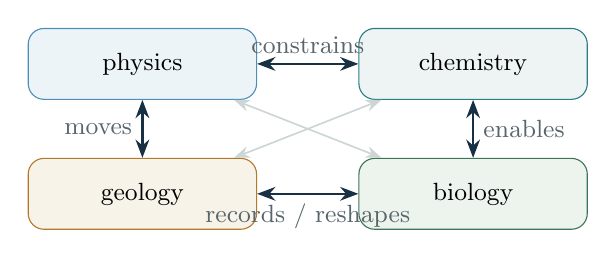
\begin{tikzpicture}[font=\small,>=Stealth]
  \node[draw=sky,fill=paleblue,rounded corners=2mm,minimum width=29mm,minimum height=9mm] (p) at (0,0) {physics};
  \node[draw=water,fill=mist,rounded corners=2mm,minimum width=29mm,minimum height=9mm] (c) at (4.2,0) {chemistry};
  \node[draw=ochre,fill=chalk,rounded corners=2mm,minimum width=29mm,minimum height=9mm] (g) at (0,-1.65) {geology};
  \node[draw=leaf,fill=palegreen,rounded corners=2mm,minimum width=29mm,minimum height=9mm] (b) at (4.2,-1.65) {biology};
  \draw[<->,line width=.8pt,night] (p)--node[above,text=slate]{constrains} (c);
  \draw[<->,line width=.8pt,night] (p)--node[left,text=slate]{moves} (g);
  \draw[<->,line width=.8pt,night] (c)--node[right,text=slate]{enables} (b);
  \draw[<->,line width=.8pt,night] (g)--node[below,text=slate]{records / reshapes} (b);
  \draw[<->,line width=.6pt,linegrey] (p)--(b);
  \draw[<->,line width=.6pt,linegrey] (c)--(g);
\end{tikzpicture}
\end{center}

Chalk is biology sedimented into geology and later interpreted through physics. Life transformed atmospheric chemistry; atmosphere and rock weathering alter waters; waters filter the light in which photosystems evolve; organisms in turn change water colour and sediment. Universal regularities operate at every step, but they do not specify which lawful sequence occurred on Earth.

Feynman made this point without exempting biology or geology from physical law. Historical sciences add the question of how the present arrangement came to be \citep{feynman1963}. Gould's famous thought experiment of replaying life's tape emphasised contingency: branching histories depend on earlier events, not only on timeless optima \citep{gould1989}. Evolution experiments make the idea testable; in one long-running bacterial population, access to a key innovation depended on earlier genetic history \citep{blount2008}.

An \term{accident} here means an event whose occurrence was not guaranteed by the general laws being invoked, and whose consequences redirected later possibilities, with no violation of law and no absence of causes anywhere in the account. A mutation can obey chemistry yet be undirected with respect to future need. A flood can obey dynamics yet remove one population and spare another. Once history turns, selection can stabilise, refine, or repurpose what contingency supplied.

An Earth-bound accident can therefore be part of a complete reason why without ever amounting to a purpose, and the word \emph{mere} deserves resistance, since contingency is frequently the very information that a historical science is trying to recover.

\section{From Kipling to ``just-so'' science}

The phrase belongs to Kipling, whose \emph{Just So Stories for Little Children} appeared in 1902 and offers playful origin tales such as how the camel got his hump \citep{kipling1902}, and attributing it correctly seems the least an essay about provenance can do. In science, a ``just-so story'' has come to mean an attractive post hoc account, especially an adaptive one, whose fit to the known outcome is easier to admire than to test. Gould and Lewontin's critique of unrestrained adaptationism made the warning famous, although the label and its uses have a more complicated history \citep{gouldlewontin1979,hubalek2020}.

The insult is often used too cheaply. Historical explanations are not defective merely because the past cannot be rerun. Geology, cosmology, and evolutionary biology constrain histories through traces, dates, phylogenies, models, comparative patterns, and experimental analogues. A story becomes scientifically strong when independent evidence makes it difficult to alter at will.

David Deutsch's useful criterion is that good explanations are \emph{hard to vary while still explaining what they purport to explain} \citep{deutsch2011}. The criterion concerns whether the details do load-bearing work, which is a separate matter from mathematical brevity or emotional austerity. If red leaves can be said to warn insects, hide from insects, attract predators of insects, protect photosystems, dispose of sugar, warm tissue, or merely accompany stress, then ``red is useful'' is not yet a discriminating explanation. Each candidate must risk different observations.

\begin{center}
\small
\renewcommand{\arraystretch}{1.24}
\begin{tabularx}{\linewidth}{>{\bfseries\color{night}}p{.22\linewidth}X}
\toprule
\textbf{Hardening move} & \textbf{Question to ask of an appealing story} \\
\midrule
Specify the contrast & Compared with which available alternative, in which lineage and environment? \\
Name the mechanism & Through which measurable links does the proposed cause reach the outcome? \\
Risk a discriminator & What result supports this account over a rival that predicts the same broad pattern? \\
Fit the chronology & Did the cause, trait, receiver, and environment overlap in time? \\
Triangulate & Do experiments, comparative data, phylogeny, and environmental reconstruction converge? \\
State the scope & Is this a local effect, a widespread tendency, or a universal claim? \\
Name a defeater & What finding would lower confidence rather than be absorbed into the story? \\
\bottomrule
\end{tabularx}
\end{center}

A textbook sentence can be true and still be too easy to vary. Adding a provenance trail and a discriminating question turns an answer-shaped vignette into the beginning of research.

\section{Four case files, honestly compressed}

The following table models short answers that can survive later decompression. Each is a well-labelled first statement, offered with its boundary attached.

\begin{center}
\footnotesize
\renewcommand{\arraystretch}{1.26}
\begin{tabularx}{\linewidth}{>{\bfseries\color{night}}p{.115\linewidth}>{\raggedright\arraybackslash}p{.245\linewidth}>{\raggedright\arraybackslash}p{.26\linewidth}X}
\toprule
\textbf{Case} & \textbf{First answer} & \textbf{Boundary} & \textbf{Invitation} \\
\midrule
Chalk & Weak visible absorption plus multiple scattering makes chalk diffusely white. & Impurities, grain size, moisture, and illumination alter appearance; this is not its geological biography. & How did biological carbonate become this rock and this classroom object? \\
\addlinespace
Blue sky & Small atmospheric molecules scatter shorter visible wavelengths strongly; human vision maps the resulting spectrum to blue. & Aerosols, clouds, solar angle, viewing direction, stellar spectrum, and observer matter. & Which part of the answer changes at sunset, on Mars, or for a different visual system? \\
\addlinespace
Natural water & Water transmits visible wavelengths relatively well but unequally; path length, particles, plankton, and dissolved matter set colour and clarity. & ``Clear'' is scale- and method-dependent; one constituent rarely explains every lake. & What would absorption, scattering, and catchment measurements each reveal? \\
\addlinespace
Green / red leaves & Pigments and tissue optics set colour. Green photons remain useful; autumn anthocyanins have several supported and disputed roles. & Present mechanism, present benefit, and historical selection require different evidence. & Which claim is secure, which is context-dependent, and which would need a phylogeny or fitness test? \\
\bottomrule
\end{tabularx}
\end{center}

The important phrase in each final column is a question whose answer would change what we are entitled to say, which does considerably more work than an admission that we do not know.

\section{A classroom practice of visible seams}

Students need recurring cues that knowledge has architecture, which a literature review appended to every sentence would never supply, and four small additions can transform an explanation while leaving it digestible.

\subsection{Inquiry needs the vignettes it interrogates}

Inquiry-based learning is often proposed as the remedy, and it is a partial one with a failure mode worth stating. An inquiry whose destination is the sanctioned vignette, reached along a worksheet that has removed every wrong turning, rehearses the appearance of discovery while delivering the same sealed sentence at greater cost in lesson time. Discernment also refuses to arrive as a transferable technique, since judging whether a claim about canopy photosynthesis is well warranted requires knowing something about canopies, and the case against minimally guided instruction rests on that dependence: novices lack the schemas that make unguided exploration productive, and cognitive load accounts for much of the rest \citep{kirschner2006}. The reply from the inquiry side is equally worth holding, namely that well-designed problem-based and inquiry sequences are heavily scaffolded and aim at epistemic practices alongside content \citep{hmelosilver2007}.

Both sides are right about different things, and the practical resolution is unglamorous. Compressed vignettes are the necessary feed, since a student with no stock of secure mechanisms has nothing to exercise discernment upon. What converts the feed into acumen is a small and repeatable addition, in which each vignette arrives with the question of what would separate it from its nearest rival, and in which a lesson occasionally spends ten minutes discovering that the textbook sentence has a boundary. Research acumen grows out of repeated exposure to that gap, slowly, in students who already know a good deal.

\subsection{The four-line explanation card}

\begin{center}
\large
\begin{tcolorbox}[width=.9\linewidth,colback=white,colframe=night,boxrule=.85pt,arc=2mm,left=5mm,right=5mm,top=3mm,bottom=3mm]
\textcolor{night}{\textbf{CLAIM}}\quad What is the smallest exact statement?\\[1.5mm]
\textcolor{water}{\textbf{WARRANT}}\quad What observation, experiment, comparison, or model supports it?\\[1.5mm]
\textcolor{autumn}{\textbf{BOUNDARY}}\quad Where, when, or at what scale might it fail?\\[1.5mm]
\textcolor{leaf}{\textbf{OPENING}}\quad What next question does the answer make possible?
\end{tcolorbox}
\end{center}

The card can sit beside a diagram, a practical, a paragraph, or an exam answer, modelled by the teacher at first and later completed or challenged by the students, with calibrated assertion as the aim and ritual caveating as the failure mode to be avoided.

\subsection{Change the assessment verb}

Questions such as ``State why leaves are green'' reward the shortest authorised vignette. Small changes demand epistemic work:

\begin{itemize}
  \item Give the best one-sentence mechanism, then identify one fact it leaves unexplained.
  \item Classify each clause as observation, mechanism, current role, history, or purpose.
  \item Compare two sources: which makes the narrower claim, and which supplies the stronger warrant?
  \item Name one observation compatible with both hypotheses and one that would separate them.
  \item Rewrite an overconfident ``because'' so its scope and confidence are visible.
\end{itemize}

These moves align with work on epistemic cognition: learners need to judge aims, sources, methods, and standards, none of which the refrain that science is ``tentative'' ever requires of them \citep{chinn2011}. They also answer a practical problem in online reasoning, where fluent presentation and institutional appearance can substitute for source evaluation \citep{mcgrew2018}.

\subsection{Teach one secure sentence and one live sentence}

For every complex case, the teacher can pair:

\begin{quote}
\textbf{Secure:} what the strongest converging evidence establishes.\\
\textbf{Live:} what researchers are still distinguishing, and what evidence would matter.
\end{quote}

For green leaves: \emph{secure}, green light is less strongly absorbed than much red and blue light, yet can drive photosynthesis deeper in tissue. \emph{Live}, which mixture of constraint, light distribution, protection, and historical contingency best explains the inherited pigment complement. For red leaves: \emph{secure}, many species synthesise anthocyanins during senescence. \emph{Live}, how much photoprotection, carbon balance, herbivore interaction, and lineage history each contributes.

This pairing prevents two symmetrical mistakes: treating the frontier as if nothing were known, and treating a settled lower-level mechanism as if every historical question had been answered.

\subsection{Make authority inspectable}

A source chain can be short:

\begin{equation*}
\text{classroom claim} \longrightarrow \text{review or synthesis} \longrightarrow \text{original data}.
\end{equation*}

Students need not follow every chain every time. They should know that the chain exists, that different links do different work, and that the teacher is willing to expose it. Accountable authority says, in effect: \emph{trust this claim in proportion to these practices, within these boundaries; here is how you could check or extend it}.

\section{A reading route for students and teachers}

The route below moves from accessible framing to research papers. For technical articles, reading the abstract, figures, captions, and discussion can be more valuable than decoding every line.

\begin{enumerate}[leftmargin=1.7em,label=\textbf{\arabic*.}]
  \item \textbf{Start with an ordinary object.} Read Weinberg's ``On a Piece of Chalk'' \citep{weinberg1992}, then sample Huxley's earlier lecture \citep{huxley1868}. Mark where each author descends towards law and where each reconstructs history.

  \item \textbf{Watch a why-question refuse to terminate.} View the magnets interview \citep{feynmanbbc1983}, then read Rosenberg on ice \citep{rosenberg2005} and the gliding measurements of \citet{canale2019}. Locate the hedge in Feynman's account, and say why his mechanism is insufficient rather than false.

  \item \textbf{Put the observer into the sky.} Read Smith's account of daylight sky colour \citep{smith2005}. Separate the scattering spectrum from the human colour response.

  \item \textbf{Turn transparency into a measurement.} Use Pope and Fry's pure-water spectrum \citep{popefry1997} and Morel and Prieur's ocean-colour analysis \citep{morel1977}. Ask what changes when the path length or constituents change.

  \item \textbf{Correct the green-light myth.} Compare classic leaf optics \citep{woolley1971} with the green-light experiments of \citet{terashima2009} and the review by \citet{liu2021}. Explain why ``looks green'' does not entail ``cannot use green''.

  \item \textbf{See a mechanism remain historically open.} Read \citet{nishio2000} on why higher plants are green. List which propositions are measurements and which are evolutionary inferences.

  \item \textbf{Enter a live biological dispute.} Contrast the photoprotection results of \citet{feild2001} and \citet{hoch2003} with the Norway maple study by \citet{mattila2023}, then use \citet{levyadun2022} to map the wider hypothesis field.

  \item \textbf{Watch a purpose bias in the laboratory.} Read the design and response items in \citet{kelemen1999}, followed by the teaching intervention in \citet{kelemen2014}. Ask what the second study prevents us from concluding from the first.

  \item \textbf{Learn to split the whys.} Read Haig's short paper \citep{haig2013} beside Tinbergen \citep{tinbergen1963}. Reclassify each ``because'' in one textbook page.

  \item \textbf{Make stories risk evidence.} Read Gould and Lewontin's adaptationism critique \citep{gouldlewontin1979} alongside Deutsch on hard-to-vary explanations \citep{deutsch2011}. Choose one appealing account and write a result that would discriminate it from a rival.

  \item \textbf{Weigh the inquiry argument.} Read \citet{kirschner2006} against \citet{hmelosilver2007}, then decide which activities in your own scheme of work supply the guidance the two sides are arguing about.

  \item \textbf{Inspect science as a knowledge practice.} Use Ford \citep{ford2008} or Allchin \citep{allchin2011} to audit one lesson: where does authority come from, where is accountability visible, and which seams could be reopened?
\end{enumerate}

\section{Coda: authority with visible seams}

Why is chalk white? Why is the sky blue? Why can one lake be transparent, another turquoise, another brown, another opaque? Why are leaves green, why do some turn red, and why is ice slippery?

Because photons meet molecules, particles, structures, paths, and observers. Because calcium carbonate accumulated in ancient seas. Because atmospheres and catchments have histories. Because chloroplasts are inherited organisations, not fresh engineering projects. Because selection can retain consequences no organism foresaw. Because lawful accidents close some paths and open others. Because a reason can be a cause or a history without being a purpose; because a function can be real without being intended; because meaning can be made without having manufactured the thing that matters.

That paragraph is broad enough to sound wise and still too compressed to teach from. Its claims have different warrants. The responsible teacher does not renounce authority; the responsible teacher shows its joints.

Ask what is left a year later, when the lesson has gone and the notes have not been opened. What survives is seldom the judgement; it is a sediment of vignettes, that pressure melts the ice, that chlorophyll reflects green, that blue is scattered most, each one a compression whose hedges, derivations, and boundary conditions were shed somewhere in transit. Compressions travel because they are cheap to carry, and a derivation is expensive, so the sentence reaches its destination while the machinery that made it trustworthy stays behind.

The familiar aphorism, that education is what remains once everything learned in school has been forgotten, is usually offered as a compliment to whoever has done the forgetting. Measured against what actually remains, it describes the sediment, and the compliment has to be earned rather than assumed.

\begin{provenance}
Einstein used the line in an address to the Convocation of the State University of New York at Albany on 15 October 1936, introducing it as somebody else's and crediting an unnamed wit \citep{einstein1950}. It has since been assigned to Skinner, to Emerson, to Conant, and to two different Lords Halifax, while a related remark about culture was circulating in the 1890s and a version was credited to Herriot by 1928 \citep{qi2014}. A sentence about what survives forgetting has itself survived by shedding the hedge that qualified it and acquiring a famous name that the man who used it declined to claim.
\end{provenance}

The image that fits a classroom is the one waiting at the end of the yellow road, where a voice of tremendous authority turns out to be a man working a console behind a curtain \citep{baum1900}. The machinery is the only substantial thing in the room, and it is also the thing nobody carries away, since a projected voice travels and a console does not. A physics education is very largely an education in machinery: how a quantity was measured, which regime an idealisation holds in, what would have counted as a refutation, whose result this was and who checked it. When the machinery is forgotten, what settles as residue is the voice.

That is an uncomfortable description of the work, and it bears directly on the idea of teaching as conveyancing, since a teacher who believes that judgement is being transferred while vignettes are being deposited has told a flattering story about their own residue.

The residue is layered, and the layers are not equally visible. On top sit the factoids, which can be recited and therefore examined. Underneath sits something no examination reaches directly, a standing disposition to ask of any confident sentence which measurement would have to come out differently for it to fail. Two students carrying identical factoids can differ completely in whether that question remains available to them, and the difference shows only when they meet a case neither has seen before. A curriculum can test the upper layer every term, and can infer the lower one only from what a student does once the vignette has run out.

Factual knowledge remains indispensable through all of this, since a learner with no stock of secure compressions has nothing to exercise discernment upon. What changes is the educational value of merely displaying it. A learner who can recite the sanctioned vignette may possess an answer while lacking an account. A learner who can state a secure mechanism, locate its boundary, inspect its provenance, distinguish present use from selected history, and formulate a question that separates rival explanations has begun to participate in science.

The purpose of a classroom answer is therefore to refine curiosity rather than to satiate it, and the best compression carries a release catch. Chalk teaches the descent towards law; sky teaches the role of the observer; water teaches scale and catchment; leaves teach function, inheritance, and contingency; ice teaches that even an exemplary explanation, delivered by an exemplary explainer, can quietly date. Each is a small curtain, and drawing it back costs a lesson very little. Knowledge loses nothing when its seams are shown, and the student who has once seen the console is the one who thinks to look behind the next voice.

\clearpage
\addcontentsline{toc}{section}{References}
\bibliographystyle{plainnat}
\bibliography{because_sources}

\end{document}
